\documentclass[9pt,twocolumn,twoside,]{pnas-new}

% Use the lineno option to display guide line numbers if required.
% Note that the use of elements such as single-column equations
% may affect the guide line number alignment.


\usepackage[T1]{fontenc}
\usepackage[utf8]{inputenc}

% tightlist command for lists without linebreak
\providecommand{\tightlist}{%
  \setlength{\itemsep}{0pt}\setlength{\parskip}{0pt}}


% Pandoc citation processing
%From Pandoc 3.1.8
% definitions for citeproc citations
\NewDocumentCommand\citeproctext{}{}
\NewDocumentCommand\citeproc{mm}{%
  \begingroup\def\citeproctext{#2}\cite{#1}\endgroup}
\makeatletter
 % allow citations to break across lines
 \let\@cite@ofmt\@firstofone
 % avoid brackets around text for \cite:
 \def\@biblabel#1{}
 \def\@cite#1#2{{#1\if@tempswa , #2\fi}}
\makeatother
\newlength{\cslhangindent}
\setlength{\cslhangindent}{1.5em}
\newlength{\csllabelwidth}
\setlength{\csllabelwidth}{3em}
\newenvironment{CSLReferences}[2] % #1 hanging-indent, #2 entry-spacing
 {\begin{list}{}{%
  \setlength{\itemindent}{0pt}
  \setlength{\leftmargin}{0pt}
  \setlength{\parsep}{0pt}
  % turn on hanging indent if param 1 is 1
  \ifodd #1
   \setlength{\leftmargin}{\cslhangindent}
   \setlength{\itemindent}{-1\cslhangindent}
  \fi
  % set entry spacing
  \setlength{\itemsep}{#2\baselineskip}}}
 {\end{list}}
\usepackage{calc}
\newcommand{\CSLBlock}[1]{#1\hfill\break}
\newcommand{\CSLLeftMargin}[1]{\parbox[t]{\csllabelwidth}{#1}}
\newcommand{\CSLRightInline}[1]{\parbox[t]{\linewidth - \csllabelwidth}{#1}\break}
\newcommand{\CSLIndent}[1]{\hspace{\cslhangindent}#1}


\templatetype{pnasresearcharticle}  % Choose template

\title{Continuous developmental changes in word recognition support
language learning across early childhood}

\author[a, 1]{Michael C. Frank}
\author[a]{Virginia A. Marchman}
\author[b]{Claire Augusta Bergey}
\author[a]{Veronica Boyce}
\author[a]{Mika Braginsky}
\author[c]{Jess Mankewitz}
\author[d]{Stephan Meylan}
\author[a]{Ben Prystawski}
\author[a, e]{Nilam Ram}
\author[a]{Robert Z. Sparks}
\author[f]{Adrian Steffan}
\author[a]{Alvin Wei Ming Tan}
\author[f]{Martin Zettersten}

  \affil[a]{Department of Psychology, Stanford University, Stanford, CA,
USA}
  \affil[b]{Department of Linguistics, Stanford University, Stanford,
CA, USA}
  \affil[c]{Department of Psychology, University of Wisconsin, Madison,
WI, USA}
  \affil[d]{Department of Linguistics, University of California,
Berkeley, CA, USA}
  \affil[e]{Department of Communication, Stanford University, Stanford,
CA, USA}
  \affil[f]{Department of Communication, Stanford University, Stanford,
CA, USA}
  \affil[g]{Department of Psychology, Ludwig Maximilian University,
Munich, Germany}


% Please give the surname of the lead author for the running footer
\leadauthor{Anonymous}

% Please add here a significance statement to explain the relevance of your work
\significancestatement{The efficiency with which children recognize
words provides a measurement of their real-time language processing,
which has been argued to be a key part of the language learning process.
Her, we use a large dataset of eye-tracking data from many different
experiments to map out the development of word recognition, finding that
this process becomes faster, more accurate, and less variable in the
period between one and six years of age, and that children who are
better at word recognition tend to have larger and faster growing
vocabularies. These data suggest that understanding language is a skill
that improves gradually with practice.}


\authorcontributions{Please provide details of author contributions
here.}



\correspondingauthor{\textsuperscript{1} To whom correspondence should
be addressed. E-mail:
\href{mailto:mcfrank@stanford.edu}{\nolinkurl{mcfrank@stanford.edu}}}

% Keywords are not mandatory, but authors are strongly encouraged to provide them. If provided, please include two to five keywords, separated by the pipe symbol, e.g:
 \keywords{  one |  two |  optional |  optional |  optional  } 

\begin{abstract}
Being a fluent language user involves recognizing words as they unfold
in time. How does this skill develop over the course of early childhood?
And how does facility in word recognition relate to the growth of
vocabulary knowledge? We address these questions using data from
Peekbank, an open database of experiments measuring children's
eye-movements during early word recognition. Combining 24 datasets from
almost 2,000 children ages 1--6 years, we show that word recognition
becomes faster, more accurate, and less variable across development.
Factor analysis reveals a cross-sectional coupling of word recognition
speed and accuracy with parent-reported vocabulary. Across a range of
models, speed, accuracy, and vocabulary also show coupled growth such
that children with faster initial word recognition tend to show faster
vocabulary growth. Together, these findings support the view that word
recognition is a skill that develops gradually across early childhood
and that this skill plays a role in supporting early language learning.
\end{abstract}

\dates{This manuscript was compiled on \today}
\doi{\url{www.pnas.org/cgi/doi/10.1073/pnas.XXXXXXXXXX}}

\begin{document}

% Optional adjustment to line up main text (after abstract) of first page with line numbers, when using both lineno and twocolumn options.
% You should only change this length when you've finalised the article contents.
\verticaladjustment{-2pt}



\maketitle
\thispagestyle{firststyle}
\ifthenelse{\boolean{shortarticle}}{\ifthenelse{\boolean{singlecolumn}}{\abscontentformatted}{\abscontent}}{}

% If your first paragraph (i.e. with the \dropcap) contains a list environment (quote, quotation, theorem, definition, enumerate, itemize...), the line after the list may have some extra indentation. If this is the case, add \parshape=0 to the end of the list environment.

\acknow{This work was supported by a grant from the Jacobs Foundation.}

\dropcap{C}hildren acquiring a language are learning a body of knowledge
-- a set of words and the ways they are combined -- but they are also
learning to deploy this knowledge in the myriad complex, noisy, and
fast-moving environments in which language is used. As children enter
their second year, language explodes onto the scene; both vocabulary and
grammatical abilities grow rapidly and in tandem (1, 2). This growth in
knowledge is also accompanied by changes in language processing
efficiency: children become quicker and more accurate in recognizing
words and matching them with their referents (3--5).

Yet unlike language production, which is manifest via overt behavior,
evidence for word recognition is often more subtle. Very young children
with incomplete knowledge may not be able to point to the correct
referent of a word, but they may still have some representation of word
meaning (6). Eye tracking has thus emerged as a key method that allows
the measurement of language comprehension with high temporal resolution:
both adults and children reliably fixate the referent of a word soon
after it is used (3, 7--10). The relative timecourse of fixation then
can provide an index of the comprehender's ability or the difference
between two stimulus conditions.

The version of this method that is used with children goes by many
names, including the intermodal preferential looking paradigm and the
``looking while listening'' paradigm (LWL, the name we adopt here) (9,
11, 12). In LWL experiments, children are typically shown a series of
trials in which two images are displayed side by side and they are asked
to find one of them. For example, a ball and a book might be shown, and
the child might hear ``Look at the ball! Can you find it?''. Accuracy is
then computed as the proportion of time they fixate the correct image
within a fixed window after the onset of the noun (``ball'' in this
case). Reaction time is computed only on trials in which the child is
fixating on the distractor image (the book) before word onset; in these
cases, the average time it takes until the child shifts fixation from
the distractor to the target is used as an index of processing speed.
Early work using this method showed that both children's speed and
accuracy increase rapidly across the second year (3, 12). Related
methods have provided a window into how children process phonological
(13), syntactic (14), and semantic (15, 16) information as well as how
their lexical representations develop (17).

Word recognition ability, as measured by LWL, is hypothesized to play a
key role in language learning. Each word that a child experiences is an
opportunity to learn; measurements of children's language input at home
are consistently associated with their vocabulary size (18, 19).
Recognizing incoming words and linking them with their referents is a
prerequisite for learning. Consider a child hearing the utterance ``Can
you put the ball in the box?'' The faster and more accurately the child
can recognize that the ball is a referent, the better they can use this
evidence to help infer the speaker's intended meaning, perhaps making
inferences about the meaning of ``put'' or ``box'' (20). Consistent with
this idea, one important study found that children's word recognition
speed mediated the relationship between home language input and
vocabulary growth (21).

\begin{table*}[ht]
\centering
\begin{tabular}{rlrrrrrrrll}
  \hline
 & dataset\_name & N subjects & N admins & Mean Age & Min Age & Max Age & Avg Trials & Avg RT Trials & CDIs & longitudinal \\ 
  \hline
1 & reflook\_v4 & 310 & 310 & 36.82 & 12.24 & 60.00 & 6.21 & 2.87 &  &  \\ 
  2 & yurovsky\_2017 & 282 & 282 & 25.64 & 12.59 & 58.65 & 5.95 & 2.79 &  &  \\ 
  3 & weaver\_zettersten\_2024 & 141 & 248 & 15.73 & 13.50 & 23.60 & 18.10 & 6.72 &  & x \\ 
  4 & fernald\_marchman\_2012 & 122 & 678 & 23.92 & 17.00 & 32.00 & 16.89 & 7.21 & x & x \\ 
  5 & sander-montant\_2022 & 122 & 122 & 21.94 & 12.02 & 31.11 & 10.07 & 4.20 & x &  \\ 
  6 & frank\_tablet\_2016 & 104 & 104 & 33.89 & 12.13 & 59.84 & 5.87 & 2.74 &  &  \\ 
  7 & baumgartner\_2014 & 100 & 100 & 12.01 & 12.00 & 13.00 & 4.00 & 2.31 & x &  \\ 
  8 & fmw\_2013 &  80 & 179 & 20.04 & 17.00 & 26.00 & 21.26 & 8.44 & x & x \\ 
  9 & adams\_marchman\_2018 &  69 & 711 & 23.58 & 13.00 & 38.00 & 18.44 & 7.92 & x & x \\ 
  10 & potter\_canine &  67 &  67 & 23.76 & 21.00 & 27.00 & 10.38 & 3.80 & x &  \\ 
  11 & fernald\_totlot &  63 & 229 & 19.68 & 15.00 & 25.00 & 15.25 & 6.06 & x & x \\ 
  12 & pomper\_prime &  63 &  63 & 39.73 & 37.90 & 42.00 & 12.98 & 5.34 &  &  \\ 
  13 & pomper\_saffran\_2016 &  60 &  60 & 44.27 & 41.00 & 47.00 & 7.55 & 3.30 &  &  \\ 
  14 & swingley\_aslin\_2002 &  50 &  50 & 15.09 & 14.13 & 16.00 & 11.74 & 3.79 & x &  \\ 
  15 & pomper\_salientme &  44 &  44 & 40.11 & 38.00 & 43.00 & 5.30 & 2.34 &  &  \\ 
  16 & perry\_cowpig &  42 &  42 & 20.45 & 19.00 & 22.00 & 14.88 & 5.43 & x &  \\ 
  17 & ronfard\_2021 &  40 &  40 & 19.95 & 18.00 & 24.00 & 18.54 & 7.62 & x &  \\ 
  18 & bacon\_gendercues &  38 &  38 & 22.87 & 22.00 & 24.00 & 18.16 & 8.00 & x &  \\ 
  19 & garrison\_bergelson\_2020 &  35 &  35 & 14.46 & 12.00 & 18.00 & 27.47 & 9.41 & x &  \\ 
  20 & pomper\_yumme &  32 &  32 & 26.38 & 25.00 & 28.00 & 7.62 & 2.31 &  &  \\ 
  21 & mahr\_coartic &  29 &  29 & 20.83 & 18.10 & 23.80 & 24.38 & 8.86 & x &  \\ 
  22 & ferguson\_eyetrackingr &  28 &  28 & 19.71 & 18.02 & 21.86 & 5.54 & 2.33 & x &  \\ 
  23 & potter\_remix &  23 &  44 & 22.59 & 18.00 & 29.00 & 6.07 & 2.58 & x & x \\ 
  24 & newman\_genderdistractor &  19 &  19 & 30.12 & 29.23 & 30.84 & 13.11 & 4.94 &  &  \\ 
  \hline
    & Total & 1963 & 3554 & 24.73 & 12.00 & 60.00 & 12.74 & 5.05 & 15 & 6 \\ 
   \hline
\end{tabular}
\caption{Characteristics of included datasets from Peekbank. `Admins` denotes separate experimental sessions. `CDIs` refers to whether the dataset contains parent report vocabulary data from the MacArthur-Bates Communicative Development Inventory.} 
\end{table*}

Word recognition speed has been used as an index of individual
differences in early childhood (4, 22--25) and beyond (26--28). Over and
above measures of vocabulary size, word recognition speed at 18 months
predicts children's standardized test scores years later (23), though
these predictions may be limited to particular ages or processing
assessments (4). Further, faster processing at 18 months is predictive
of whether ``late talkers'' catch up to their peers or require further
intervention (24). Critically, all of these assessments use words that
children are reported to understand and produce -- they are not indices
of vocabulary size but rather of how quickly and accurately they can
recognize a spoken word and use it to guide their visual attention to a
referent.

Yet individual experiments measuring processing with young children
typically recruit relatively small samples in a restricted range of
ages. These samples provide neither the breadth of ages nor the number
of participants needed to estimate the broader dynamics of how word
recognition changes developmentally and how it connects with other
aspects of language {[}as has been done with school-aged children; (26);
(28){]}. Here we investigate two hypotheses.

First, one influential theory characterizes language learning as a
process of learning the skill of real-time processing (29, 30). Based on
this theory, we should expect to see the signatures of expertise and
skill learning in word recognition. Accuracy should change linearly with
the logarithm of age, reflecting gradual asymptotic convergence to
mature levels of accuracy. In addition, the logarithm of processing
speed should decrease with the logarithm of age, potentially reflecting
the ``power law of practice'' (31--33, cf 34). Finally, trial-to-trial
variability in both speed and accuracy should decrease with increasing
expertise (35).

Second, previous findings have provided limited and sometimes
conflicting evidence on the concurrent and predictive relations between
word recognition and language learning. Initial reports showed strong
predictive relationships between both speed and accuracy and later
vocabulary growth (22), with replications in infants born preterm (36)
and late talkers (24). Subsequent studies have primarily focused on
speed of processing and found more mixed results, with reaction time
measures found to be only inconsistently predictive of later vocabulary
outcomes (4, 25, 37). To the extent that there are consistent relations
between vocabulary and word recognition, these should be visible in a
larger dataset. Further, by examining the relationship between speed,
accuracy, and vocabulary, it should be possible to assess the extent to
which processing speed specifically plays a role in vocabulary growth.

\section*{Results}\label{results}
\addcontentsline{toc}{section}{Results}

To address these questions, we made use of a new release of data in
Peekbank, an open database of LWL from young children, stored in a
harmonized format (38). We retrieved data from children ages 1--6 years.
Although experiments in Peekbank include a variety of different
experimental manipulations, we analyzed data only from simple word
recognition trials in which children were shown two pictures of concrete
objects and heard a label for an object (typically embedded in a simple
carrier phrase such as ``Look at the \ldots{}''); these trials often
constituted control conditions for experiments. We focus here on English
purely for practical reasons -- the Peekbank dataset contains limited
data from other languages.

These criteria yielded 24 datasets, including 1963 children and 3554
administrations of the LWL procedure (some datasets were longitudinal or
involved multiple closely-spaced testing sessions). Table
\ref{tab:datasets} shows the characteristics of individual datasets (see
also Figures S1 and S2). The size of the combined dataset, the unified
data processing pipeline, and the fact that individual studies used very
similar implementations of the LWL experimental paradigm, all allowed us
to make a more detailed study of the development of word recognition
than has previously been possible. While our analysis is exploratory in
nature, it is guided by the two hypotheses outlined above: the presence
of 1) signatures of skill learning in word recognition, and 2) linkages
between word recognition and vocabulary.

\subsection*{Speed and accuracy of word recognition
increase}\label{speed-and-accuracy-of-word-recognition-increase}
\addcontentsline{toc}{subsection}{Speed and accuracy of word recognition
increase}

We began by characterizing developmental changes in speed and accuracy.
We computed both RTs (reaction times) and accuracies following standard
practices in the literature (9). Because there is no consensus about the
length of time windows for the computation of accuracy, we considered
both a shorter window (from 200 -- 2200 ms after noun onset) and a
longer window (from 200 -- 4000 ms). For each window, we averaged all
fixation within the window to compute a continuous proportion between 0
(no fixation on the target during the window) and 1 (total fixation on
the target during the window) on every trial.

Our first question was about the functional form of the relationships
between age, speed, and accuracy (see SI for raw correlations between
variables). To investigate this question, we fit linear mixed effects
models predicting accuracy and RT on each trial across the full dataset
with random slopes of child age by study and random intercepts by
participant. We compared models that included both long and short
accuracy windows, as well as logarithmic and linear effects of age, and
logarithmic and linear transformations of RT. The best fitting model of
accuracy predicted long window accuracy as a function of the logarithm
of age,\footnote{This longer window yielded overall higher cross-trial
  reliability as well, and so we report long window results in the main
  text. All findings reported here hold for both window sizes, however
  (see SI).} and the best fitting model of speed predicted log RT as a
function of log age as well (see SI).

Figure \ref{fig:devchange} shows these relationships. Log RT decreased
significantly with age (\(\hat{\beta} = -0.11\), 95\% CI
\([-0.14, -0.08]\), \(t(12.86) = -8.39\), \(p < .001\)) and accuracy
increased significantly with age (\(\hat{\beta} = 0.07\), 95\% CI
\([0.06, 0.08]\), \(t(17.34) = 12.77\), \(p < .001\)). In sum, we see
continuing improvements in word recognition across the full age range in
our dataset that appear roughly linear in the logarithm of age. These
logarithmic relationships follow theoretical expectations that both
speed and accuracy should gradually asymptote to mature levels of
performance as in skill learning more generally (31).

\begin{figure*}
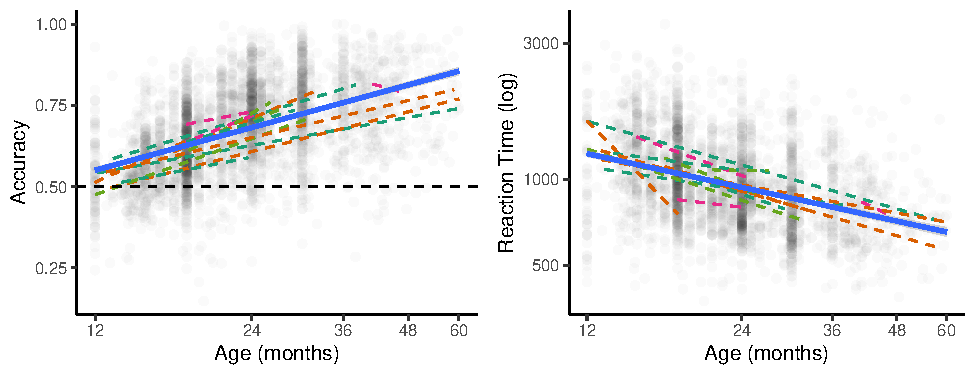
\includegraphics{paper_files/figure-latex/devchange-1} \caption{Participant-level accuracy and reaction time (log), plotted by age (log). The solid blue line shows a linear fit and associated confidence interval. Individual dotted lines show linear fits for those datasets spanning six or more months of age. The dashed line for accuracy shows chance-level looking (.5)}\label{fig:devchange}
\end{figure*}

\subsection*{Variability of word recognition
decreases}\label{variability-of-word-recognition-decreases}
\addcontentsline{toc}{subsection}{Variability of word recognition
decreases}

One further hallmark of increasing skill is a decrease in task-relevant
variability (35). Both within and across datasets, within-individual
variation in accuracy and RT decreased smoothly across the developmental
range we examined (Figure \ref{fig:variance}). We fit mixed effects
models to the standard deviation of both accuracy and RT for each
testing session for each participant, including random slopes of log age
by dataset and random intercepts for each participant. For both speed
and accuracy, within-individual variability decreased with age (RT:
\(\hat{\beta} = -0.03\), 95\% CI \([-0.05, -0.02]\),
\(t(12.48) = -5.30\), \(p < .001\); accuracy: \(\hat{\beta} = -0.03\),
95\% CI \([-0.04, -0.03]\), \(t(13.52) = -11.90\), \(p < .001\)). Thus,
as well as being faster and more accurate, older children were more
consistent in their online word recognition.

\begin{figure*}
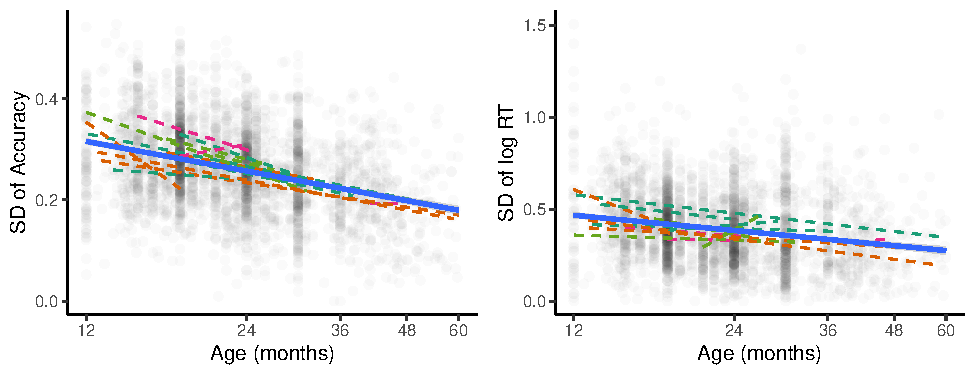
\includegraphics{paper_files/figure-latex/variance-1} \caption{Participant-level variability in accuracy and reaction time (log RT), plotted by age (log). Plotting conventions are as in Figure 1.}\label{fig:variance}
\end{figure*}

\subsection*{Speed and accuracy relate to vocabulary
size}\label{speed-and-accuracy-relate-to-vocabulary-size}
\addcontentsline{toc}{subsection}{Speed and accuracy relate to
vocabulary size}

We were next interested in whether the various aspects of word
recognition -- including accuracy, RT, and the variability of each of
these -- were related to other aspects of early language ability. Of the
studies in our database, 16 gathered parent reports about children's
early vocabulary using the MacArthur-Bates Communicative Development
Inventory (CDI), a popular survey instrument that provides a reliable
and valid estimate of children's early vocabulary (2, 39). Different
forms of the CDI can be used to measure either receptive and expressive
vocabulary (for children up to 18 months) or expressive vocabulary only
(for children 16 -- 30 months).

We fit a series of factor analytic models to explore the dimensionality
of the data. Initial exploratory factor analysis using parallel analysis
suggested that three factors explained substantial variance in the data
(see SI: Factor Analysis). Due to missingness of data, we used
confirmatory factor analysis with full information maximum likelihood to
find the best set of loadings. The best fitting model was a three-factor
model with factors for speed (RT and RT variability), accuracy (accuracy
and accuracy variability), and vocabulary (comprehension and production
from the CDI). Fit statistics for this model were generally good
(Confirmatory fit index: 0.975, RMSE: 0.06); see SI: Alternative Factor
Structures).

\begin{figure*}
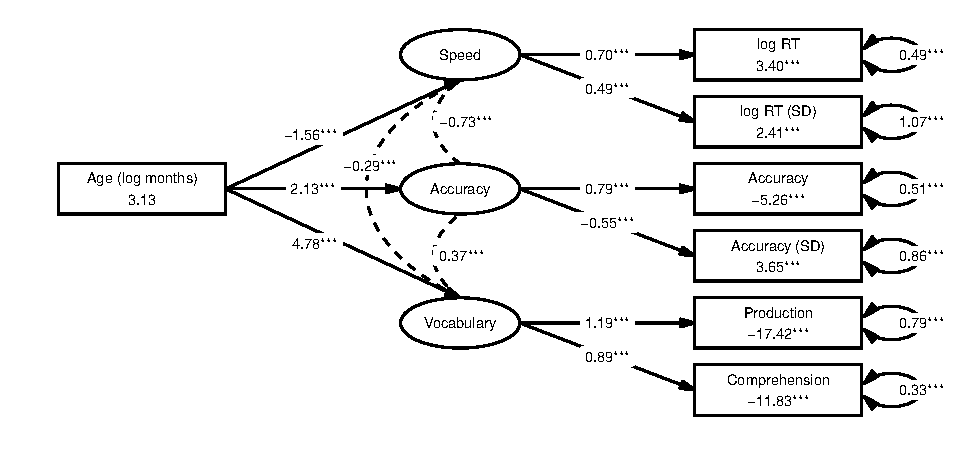
\includegraphics{paper_files/figure-latex/age_regression-1} \caption{Structural equation model showing the three-factor factor analysis with a regression of each latent variable on the logarithm of age. Observed variables are notated as squares and latent variables are notated as circles Factor loadings and regression coefficients are shown with straight, solid lines; covariances are shown with dashed lines; residual variances are shown as solid circular connections. Stars show conventional levels of statistical significance, e.g. * indicates p < .05, ** indicates p < .01, and *** indicates p < .001. Covariances reflect age-residualized correlations between variables. Abbreviations: acc = accuracy, prod = production vocabulary, comp = comprehension vocabulary.}\label{fig:age_regression}
\end{figure*}

Figure \ref{fig:age_regression} shows a regression model fit to this
confirmatory factor analysis, with log age predicting each latent
variable. This regression model allows interpretation of the covariances
between latent factors as partial correlations (controlling for age).
All three latent factors were significantly related to one another, with
RT and accuracy showing strong negative covariance (\(\beta=\) -0.734,
SE = 0.034, \(p < .0001\)) and weaker but significant covariation
between RT and vocabulary (\(\beta=\) -0.294, SE = 0.036, \(p < .0001\))
and accuracy and vocabulary (\(\beta=\) 0.369, SE = 0.033,
\(p < .0001\)). This model supports the idea that individual variation
in speed and accuracy of word recognition is concurrently related to
vocabulary beyond the effects of age.

\subsection*{Speed of processing relates to vocabulary
growth}\label{speed-of-processing-relates-to-vocabulary-growth}
\addcontentsline{toc}{subsection}{Speed of processing relates to
vocabulary growth}

While we fit the latent variable models above to the full
cross-sectional dataset, we were most interested in within-child
developmental changes, as measured within individual studies. To probe
these changes, we first examined test-retest reliability for our primary
variables of interest by calculating Pearson correlations between pairs
of administrations given no more than three months apart. Test-retest
correlations were significant but relatively modest
(\(\rho_{acc} = 0.455\), \(\rho_{rt} =  0.407\)), suggesting that,
across studies, LWL measures from individual sessions provide relatively
noisy measurements of individual children even if individual studies are
able to achieve higher reliability by averaging across measurement
occasions (e.g., 23).

Given this relatively low reliability in our longitudinal datasets
(which also tended to be from younger children), we chose to measure
relationships between LWL and vocabulary using longitudinal growth
models. We began by reproducing the analysis reported in (24), in which
longitudinal growth in productive vocabulary was predicted based on RT
during the initial session of the study. We fit a mixed effects model
predicting growth in vocabulary as a quadratic function of age, RT at
study initiation (\(t_0\)), and their interaction (as well as random
effects of age by participant and by dataset). This model revealed a
significant effect of \(t_0\) RT (\(\hat{\beta} = -0.14\), 95\% CI
\([-0.21, -0.06]\), \(t(294.12) = -3.61\), \(p < .001\)) and an
interaction between \(t_0\) RT and the quadratic age predictor
(\(\hat{\beta} = 1.44\), 95\% CI \([0.76, 2.11]\),
\(t(1036.95) = 4.15\), \(p < .001\)). This analysis suggests that
children with faster initial RTs show both larger vocabularies and
faster vocabulary growth over time, confirming that findings from (24)
were robust across the full dataset.

On the other hand, it is possible that differences in predicted growth
trajectories are due to overall coupling between vocabulary size and
language processing, rather than a specifically predictive relationship
between \(t_0\) RT and vocabulary growth. To test this relationship, we
used longitudinal structural equation models. We separated the
longitudinal speed, accuracy, and vocabulary data into two-month bins
spanning up to 10 months (\(t_0 ... t_4\)) and fit individual growth
across each of these variables. We used full-information maximum
likelihood to handle the substantial missing data caused by the
different longitudinal sampling schemes of studies in our dataset. (We
present a model of coupled growth in the observed variables here for
simplicity; see SI for a comparable model using growth in the latent
factors). The fitted longitudinal model is shown in Figure
\ref{fig:longitudinal}. Overall fit statistics were generally acceptable
(Confirmatory fit index: 0.883, RMSE: 0.028, RMSE \(p\)-value: 1).

Our key question of interest concerned coupling between the parameters
of these growth models. Consistent with the idea that overall faster
processing is related to vocabulary growth, we saw significant coupling
between processing speed intercepts and vocabulary growth slopes
(\(\beta=\) -0.136, SE = 0.052, \(p =\) 0.008) as well as a variety of
other couplings. There was not significant coupling between growth in RT
and growth in vocabulary (\(\beta=\) -0.006, SE = 0.014, \(p =\) 0.674).
These abilities might grow independently, but we cannot rule out other
possibilities. First, the longitudinal data we had might not allow
sufficiently precise estimates of growth slopes, or second, since
vocabulary growth is non-linear, the linear model we used here might not
be as sensitive to non-linear changes.

In sum, these findings provide further evidence consistent with the
claim that faster processing is related to longitudinal growth in
vocabulary (21, 22). Children with greater skill in word recognition
learn words faster.

\begin{figure*}
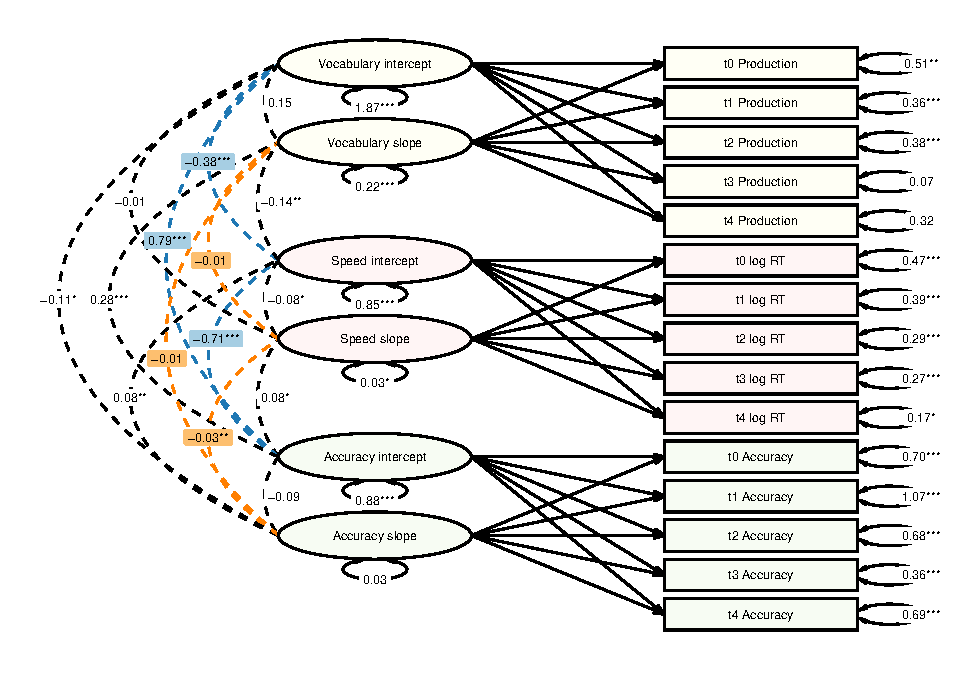
\includegraphics{paper_files/figure-latex/longitudinal-1} \caption{Structural equation model showing longitudinal couplings between growth parameters. }\label{fig:longitudinal}
\end{figure*}

\section*{Discussion}\label{discussion}
\addcontentsline{toc}{section}{Discussion}

How does word recognition change across early childhood and how does it
relate to language learning? We investigated these questions using a
new, large-scale dataset of developmental eye-tracking measurements
compiled across many prior studies. We found continuous developmental
changes from ages 1 -- 6 years. Speed and accuracy both improved
asymptotically, with evidence that recognition speed showed the log-log
relationship associated with the ``power law of practice'', that is,
gradually converging on mature levels of processing efficiency. Further,
trial-to-trial variability decreased, consistent with both the
literature on skill learning (35) and other work on developmental
changes in variability (40--42). Speed and accuracy were both related to
vocabulary size concurrently and processing speed was also related to
later vocabulary growth.

Together, our findings are consistent with theories that posit that
language learning is a process of skill acquisition, in which children
become adept at quickly converting ephemeral signals into meaning (29).
This skill develops gradually over the course of early childhood and
supports word learning. Further, our results point to consistency
between skill development in early childhood and the continued
refinement of language processing and language knowledge during middle
childhood (26, 28).

By aggregating data from many pre-existing studies, we were able to
overcome the limitations of prior investigations, which typically had
sample sizes at least an order of magnitude smaller than ours. In
contrast to individual studies, which typically have at best the
statistical power to test one or two specific contrasts, our ``big
data'' approach provided the sample sizes necessary to fit complex
structural equation models and to compare different functional forms for
developmental change. Because early language is so variable (2), these
kinds of samples -- with thousands, rather than dozens of children --
are likely to be required to gain further insight into the psychometrics
of early language learning
{[}\href{mailto:bergelson2023;@frank2017}{\nolinkurl{bergelson2023;@frank2017}};(2);(43){]}.

At the same time, our approach is both observational and exploratory.
Thus, we cannot untangle the range of different causal models that
explain the variation we observed. First, early word recognition skill
could lead to faster word learning, due to skilled children gleaning
more information from the same signal (22). But second, faster children
could also be faster due to their larger vocabulary and stronger lexical
representations. These two causal directions could also interact
reciprocally, leading to a ``rich get richer'' process in which children
with larger vocabularies process faster, and their faster processing
helps them increase their vocabulary size more rapidly. Finally, a third
shared factor -- perhaps general cognitive ability -- could underpin
both processes. Our cross-sectional data cannot distinguish these
hypotheses even in principle (44), and our longitudinal data are likely
too sparse to distinguish such complex causal models. Thus, these
questions remain an open target for dense longitudinal data collection.

Our findings here are limited in their generalizability by the
convenience samples that were used in the individual studies in the
Peekbank database. These studies typically (but not always) represent
children from well-educated parents living in university-adjacent
communities. We would not expect that specific numerical parameters
estimated in this aggregate convenience sample would generalize to other
samples. Nevertheless, the consistency of the trends we observed across
datasets suggests that our qualitative conclusions are robust to some
significant sociodemographic variation.

More broadly, our results here suggest the continued importance of the
looking-while-listening paradigm as an index of children's language
processing abilities. If language learning is, at least in part, a
process of skill learning, then measurement of this skill is a critical
window into understanding the remarkable process of language learning.

\showmatmethods
\showacknow
\pnasbreak

\newpage

\phantomsection\label{refs}
\begin{CSLReferences}{0}{1}
\bibitem[\citeproctext]{ref-bates1994developmental}
\CSLLeftMargin{1. }%
\CSLRightInline{Bates E, et al. (1994) Developmental and stylistic
variation in the composition of early vocabulary. \emph{Journal of child
language} 21(1):85--123.}

\bibitem[\citeproctext]{ref-frank2021}
\CSLLeftMargin{2. }%
\CSLRightInline{Frank MC, Braginsky M, Yurovsky D, Marchman VA (2021)
\emph{{Variability and Consistency in Early Language Learning: The
Wordbank Project}} (MIT Press, Cambridge, MA).}

\bibitem[\citeproctext]{ref-fernald1998}
\CSLLeftMargin{3. }%
\CSLRightInline{Fernald A, Pinto JP, Swingley D, Weinberg A, McRoberts
GW (1998) Rapid gains in speed of verbal processing by infants in the
2nd year. \emph{Psychological Science} 9(3):228--231.}

\bibitem[\citeproctext]{ref-peter2019}
\CSLLeftMargin{4. }%
\CSLRightInline{Peter MS, et al. (2019) Does speed of processing or
vocabulary size predict later language growth in toddlers?
\emph{Cognitive Psychology} 115:101238.}

\bibitem[\citeproctext]{ref-bergelson2020comprehension}
\CSLLeftMargin{5. }%
\CSLRightInline{Bergelson E (2020) The comprehension boost in early word
learning: Older infants are better learners. \emph{Child development
perspectives} 14(3):142--149.}

\bibitem[\citeproctext]{ref-bergelson2012}
\CSLLeftMargin{6. }%
\CSLRightInline{Bergelson E, Swingley D (2012)
\href{https://www.ncbi.nlm.nih.gov/pubmed/22331874}{{At 6-9 months,
human infants know the meanings of many common nouns.}}
\emph{Proceedings of the National Academy of Sciences}
109(9):3253--3258.}

\bibitem[\citeproctext]{ref-tanenhaus1995integration}
\CSLLeftMargin{7. }%
\CSLRightInline{Tanenhaus MK, Spivey-Knowlton MJ, Eberhard KM, Sedivy JC
(1995) Integration of visual and linguistic information in spoken
language comprehension. \emph{Science} 268(5217):1632--1634.}

\bibitem[\citeproctext]{ref-altmann1999incremental}
\CSLLeftMargin{8. }%
\CSLRightInline{Altmann GT, Kamide Y (1999) Incremental interpretation
at verbs: Restricting the domain of subsequent reference.
\emph{Cognition} 73(3):247--264.}

\bibitem[\citeproctext]{ref-fernald2008}
\CSLLeftMargin{9. }%
\CSLRightInline{Fernald A, Zangl R, Portillo AL, Marchman VA (2008)
{Looking while listening: Using eye movements to monitor spoken language
comprehension by infants and young children}. \emph{Developmental
Psycholinguistics: On-Line Methods in Children's Language Processing},
eds Sekerina IA, Fernandez EM, Clahsen H (John Benjamins, Amsterdam), pp
97--135.}

\bibitem[\citeproctext]{ref-macdonald2018}
\CSLLeftMargin{10. }%
\CSLRightInline{MacDonald K, LaMarr T, Corina D, Marchman VA, Fernald A
(2018) Real-time lexical comprehension in young children learning
american sign language. \emph{Developmental science} 21(6):e12672.}

\bibitem[\citeproctext]{ref-hirsh1996intermodal}
\CSLLeftMargin{11. }%
\CSLRightInline{Hirsh-Pasek K, Golinkoff RM (1996) The intermodal
preferential looking paradigm: A window onto emerging language
comprehension.}

\bibitem[\citeproctext]{ref-reznick1990visual}
\CSLLeftMargin{12. }%
\CSLRightInline{Reznick JS (1990) Visual preference as a test of infant
word comprehension. \emph{Applied Psycholinguistics} 11(2):145--166.}

\bibitem[\citeproctext]{ref-mani2011}
\CSLLeftMargin{13. }%
\CSLRightInline{Mani N, Plunkett K (2011) Phonological priming and
cohort effects in toddlers. \emph{Cognition} 121(2):196--206.}

\bibitem[\citeproctext]{ref-trueswell1999kindergarten}
\CSLLeftMargin{14. }%
\CSLRightInline{Trueswell JC, Sekerina I, Hill NM, Logrip ML (1999) The
kindergarten-path effect: Studying on-line sentence processing in young
children. \emph{Cognition} 73(2):89--134.}

\bibitem[\citeproctext]{ref-mani2010}
\CSLLeftMargin{15. }%
\CSLRightInline{Mani N, Plunkett K (2010) In the infant's mind's ear:
Evidence for implicit naming in 18-month-olds. \emph{Psychological
science} 21(7):908--913.}

\bibitem[\citeproctext]{ref-bergelson2017}
\CSLLeftMargin{16. }%
\CSLRightInline{Bergelson E, Aslin RN (2017) Nature and origins of the
lexicon in 6-mo-olds. \emph{Proceedings of the National Academy of
Sciences} 114(49):12916--12921.}

\bibitem[\citeproctext]{ref-Swingley2002}
\CSLLeftMargin{17. }%
\CSLRightInline{Swingley D, Aslin RN (2002)
\href{https://doi.org/10.1111/1467-9280.00485}{{Lexical neighborhoods
and the word-form representations of 14-month-olds}}.
\emph{Psychological Science} 13(5):480--484.}

\bibitem[\citeproctext]{ref-hart1995meaningful}
\CSLLeftMargin{18. }%
\CSLRightInline{Hart B, Risley TR (1995) Meaningful differences in the
everyday experience of young american children.}

\bibitem[\citeproctext]{ref-anderson2021linking}
\CSLLeftMargin{19. }%
\CSLRightInline{Anderson NJ, Graham SA, Prime H, Jenkins JM, Madigan S
(2021) Linking quality and quantity of parental linguistic input to
child language skills: A meta-analysis. \emph{Child Development}
92(2):484--501.}

\bibitem[\citeproctext]{ref-frank2009using}
\CSLLeftMargin{20. }%
\CSLRightInline{Frank MC, Goodman ND, Tenenbaum JB (2009) Using
speakers' referential intentions to model early cross-situational word
learning. \emph{Psychological science} 20(5):578--585.}

\bibitem[\citeproctext]{ref-Weisleder2013}
\CSLLeftMargin{21. }%
\CSLRightInline{Weisleder A, Fernald A (2013)
\href{https://doi.org/10.1177/0956797613488145}{{Talking to children
matters: Early language experience strengthens processing and builds
vocabulary}}. \emph{Psychological Science} 24(11):2143--2152.}

\bibitem[\citeproctext]{ref-fernald2006}
\CSLLeftMargin{22. }%
\CSLRightInline{Fernald A, Perfors A, Marchman VA (2006) Picking up
speed in understanding: Speech processing efficiency and vocabulary
growth across the 2nd year. \emph{Developmental psychology} 42(1):98.}

\bibitem[\citeproctext]{ref-marchman2008}
\CSLLeftMargin{23. }%
\CSLRightInline{Marchman VA, Fernald A (2008)
\href{https://www.ncbi.nlm.nih.gov/pubmed/18466367}{{Speed of word
recognition and vocabulary knowledge in infancy predict cognitive and
language outcomes in later childhood.}} \emph{Developmental science}
11(3):F9--16.}

\bibitem[\citeproctext]{ref-fernald2012}
\CSLLeftMargin{24. }%
\CSLRightInline{Fernald A, Marchman VA (2012)
\href{https://www.ncbi.nlm.nih.gov/pubmed/22172209}{{Individual
differences in lexical processing at 18 months predict vocabulary growth
in typically developing and late-talking toddlers.}} \emph{Child
development} 83(1):203--22.}

\bibitem[\citeproctext]{ref-newbury2016interrelationships}
\CSLLeftMargin{25. }%
\CSLRightInline{Newbury J, Klee T, Stokes SF, Moran C (2016)
Interrelationships between working memory, processing speed, and
language development in the age range 2--4 years. \emph{Journal of
Speech, Language, and Hearing Research} 59(5):1146--1158.}

\bibitem[\citeproctext]{ref-colby2023efficiency}
\CSLLeftMargin{26. }%
\CSLRightInline{Colby SE, McMurray B (2023) Efficiency of spoken word
recognition slows across the adult lifespan. \emph{Cognition}
240:105588.}

\bibitem[\citeproctext]{ref-jeppsen2022development}
\CSLLeftMargin{27. }%
\CSLRightInline{Jeppsen C, Baxelbaum K, Tomblin B, Klein K, McMurray B
(2022) The development of lexical processing: Real-time phonological
competition and semantic activation in school age children.
\emph{Quarterly Journal of Experimental Psychology}:17470218241244799.}

\bibitem[\citeproctext]{ref-mcmurray2022slow}
\CSLLeftMargin{28. }%
\CSLRightInline{McMurray B, Apfelbaum KS, Tomblin JB (2022) The slow
development of real-time processing: Spoken-word recognition as a
crucible for new thinking about language acquisition and language
disorders. \emph{Current Directions in Psychological Science}
31(4):305--315.}

\bibitem[\citeproctext]{ref-christiansen2016}
\CSLLeftMargin{29. }%
\CSLRightInline{Christiansen MH, Chater N (2016) The now-or-never
bottleneck: A fundamental constraint on language. \emph{Behavioral and
brain sciences} 39:e62.}

\bibitem[\citeproctext]{ref-chater2018}
\CSLLeftMargin{30. }%
\CSLRightInline{Chater N, Christiansen MH (2018) Language acquisition as
skill learning. \emph{Current opinion in behavioral sciences}
21:205--208.}

\bibitem[\citeproctext]{ref-snoddy1926}
\CSLLeftMargin{31. }%
\CSLRightInline{Snoddy GS (1926) Learning and stability: A
psychophysiological analysis of a case of motor learning with clinical
applications. \emph{Journal of Applied Psychology} 10(1):1.}

\bibitem[\citeproctext]{ref-kail1991}
\CSLLeftMargin{32. }%
\CSLRightInline{Kail R (1991) Processing time declines exponentially
during childhood and adolescence. \emph{Developmental psychology}
27(2):259.}

\bibitem[\citeproctext]{ref-anderson1982}
\CSLLeftMargin{33. }%
\CSLRightInline{Anderson JR (1982) Acquisition of cognitive skill.
\emph{Psychological review} 89(4):369.}

\bibitem[\citeproctext]{ref-heathcote2000}
\CSLLeftMargin{34. }%
\CSLRightInline{Heathcote A, Brown S, Mewhort DJ (2000) The power law
repealed: The case for an exponential law of practice. \emph{Psychonomic
bulletin \& review} 7(2):185--207.}

\bibitem[\citeproctext]{ref-todorov2002optimal}
\CSLLeftMargin{35. }%
\CSLRightInline{Todorov E, Jordan MI (2002) Optimal feedback control as
a theory of motor coordination. \emph{Nature neuroscience}
5(11):1226--1235.}

\bibitem[\citeproctext]{ref-marchman2016}
\CSLLeftMargin{36. }%
\CSLRightInline{Marchman VA, Adams KA, Loi EC, Fernald A, Feldman HM
(2016) Early language processing efficiency predicts later receptive
vocabulary outcomes in children born preterm. \emph{Child
Neuropsychology} 22(6):649--665.}

\bibitem[\citeproctext]{ref-lany2018}
\CSLLeftMargin{37. }%
\CSLRightInline{Lany J (2018) Lexical-processing efficiency leverages
novel word learning in infants and toddlers. \emph{Developmental
science} 21(3):e12569.}

\bibitem[\citeproctext]{ref-zettersten2023peekbank}
\CSLLeftMargin{38. }%
\CSLRightInline{Zettersten M, et al. (2023) Peekbank: An open,
large-scale repository for developmental eye-tracking data of children's
word recognition. \emph{Behavior Research Methods} 55(5):2485--2500.}

\bibitem[\citeproctext]{ref-marchman2023}
\CSLLeftMargin{39. }%
\CSLRightInline{Marchman VA, Dale PS, Fenson L (2023)
\emph{MacArthur-bates communicative development inventories userś guide
and technical manual, third edition} (Brookes).}

\bibitem[\citeproctext]{ref-judd2021working}
\CSLLeftMargin{40. }%
\CSLRightInline{Judd N, Klingberg T, Sjöwall D (2021) Working memory
capacity, variability, and response to intervention at age 6 and its
association to inattention and mathematics age 9. \emph{Cognitive
Development} 58:101013.}

\bibitem[\citeproctext]{ref-galeano2018variability}
\CSLLeftMargin{41. }%
\CSLRightInline{Galeano Weber EM, Dirk J, Schmiedek F (2018) Variability
in the precision of children's spatial working memory. \emph{Journal of
Intelligence} 6(1):8.}

\bibitem[\citeproctext]{ref-kautto2023introducing}
\CSLLeftMargin{42. }%
\CSLRightInline{Kautto A, Railo H, Mainela-Arnold E (2023) Introducing
the intra-individual variability hypothesis in explaining individual
differences in language development.}

\bibitem[\citeproctext]{ref-manybabies2020}
\CSLLeftMargin{43. }%
\CSLRightInline{The ManyBabies Consortium (2020) {Quantifying sources of
variability in infancy research using the infant-directed speech
preference}. \emph{Advances in Methods and Practices in Psychological
Science} 3(1):24--52.}

\bibitem[\citeproctext]{ref-vanderweele2023dimensional}
\CSLLeftMargin{44. }%
\CSLRightInline{VanderWeele TJ, Batty CJ (2023) On the dimensional
indeterminacy of one-wave factor analysis under causal effects.
\emph{Journal of Causal Inference} 11(1):20220074.}

\end{CSLReferences}



% Bibliography
% \bibliography{pnas-sample}

\end{document}
